\documentclass[12pt]{article}
\usepackage[italian]{babel}
\usepackage[utf8x]{inputenc}
\usepackage{amsmath}
\usepackage{graphicx}
\usepackage[colorinlistoftodos]{todonotes}

\begin{document}
	\begin{titlepage}
			\newcommand{\HRule}{\rule{\linewidth}{0.5mm}} % Defines a new command for the horizontal lines, change thickness here
		
		\center % Center everything on the page
		
		%----------------------------------------------------------------------------------------
		%	HEADING SECTIONS
		%----------------------------------------------------------------------------------------
		
		\textsc{\LARGE Università degli studi di Padova}\\[1.5cm] % Name of your university/college
		
\includegraphics[scale=0.3]{images/unipd_logo.png}\\[1cm] % Include a department/university logo - this will require the graphicx package
		\textsc{\Large Relazione progetto per il corso di Web Information Management}\\[0.5cm] % Major heading such as course name
		\textsc{\large Corso di Laurea in Informatica, A.A. 2016-2017}\\[0.5cm] % Minor heading such as course title
		%----------------------------------------------------------------------------------------
		%	TITLE SECTION
		%----------------------------------------------------------------------------------------
		
		\HRule \\[0.4cm]
		{ \huge \bfseries Analisi usabilità strumentimusicali.net}\\[0.4cm] % Title of your document
		\HRule \\[1.5cm]
		
		%----------------------------------------------------------------------------------------
		%	AUTHOR SECTION
		%----------------------------------------------------------------------------------------
			\begin{minipage}{0.4\textwidth}
				\begin{flushleft} \large
					\emph{Studente:}\\
				 Matteo Slanzi \\ \#1100866
				\end{flushleft}
			\end{minipage}
			~
			\begin{minipage}{0.4\textwidth}
				\begin{flushright} \large
					\emph{Docente:} \\
					Massimo Marchiori
				\end{flushright}
			\end{minipage}\\[2cm]
		
		
		\vfill % Fill the rest of the page with whitespace
	\end{titlepage}
	\newpage
	\renewcommand{\contentsname}{Indice}
	\tableofcontents
	
	\newpage
	\section{Introduzione}
	\vspace {0.5cm}
	Il progetto riguardante il corso di Web Information Management consiste nell'analisi di usabilità di un sito web.\\ La mia scelta riguarda un sito di e-commerce di strumenti musicali che vende, principalmente in Italia, una vasta gamma di strumenti e accessori musicali, sia professionali che amatoriali. 
	\\
	Il sito mi è sembrato fin da subito ben fatto e ho deciso di analizzarlo, anche per via di un acquisto di un paio di cuffie fatto qualche mese fa.
	\newpage
	\section{Analisi delle pagine}
		\subsection{Homepage}
	La homepage del sito è molto ricca, nell'header troviamo subito il logo del sito, il menu, la barra di ricerca e lo slideshow che mostra gli articoli in sconto o novità. Più sotto troviamo gli articoli in evidenza, gli ultmi arrivi del mese, ultime recensioni e news. In fondo, il footer raggruppa diverse informazioni quali, l'assistenza post vendita, le modalità di pagamento e consegna, diritti e privacy, link ai vari social e tutte le informazione dell'azienda che si occupa della gestione e vendita dei prodotti del sito.
	\vspace{1cm}
	\begin{figure}[ht!]
		\centering	
		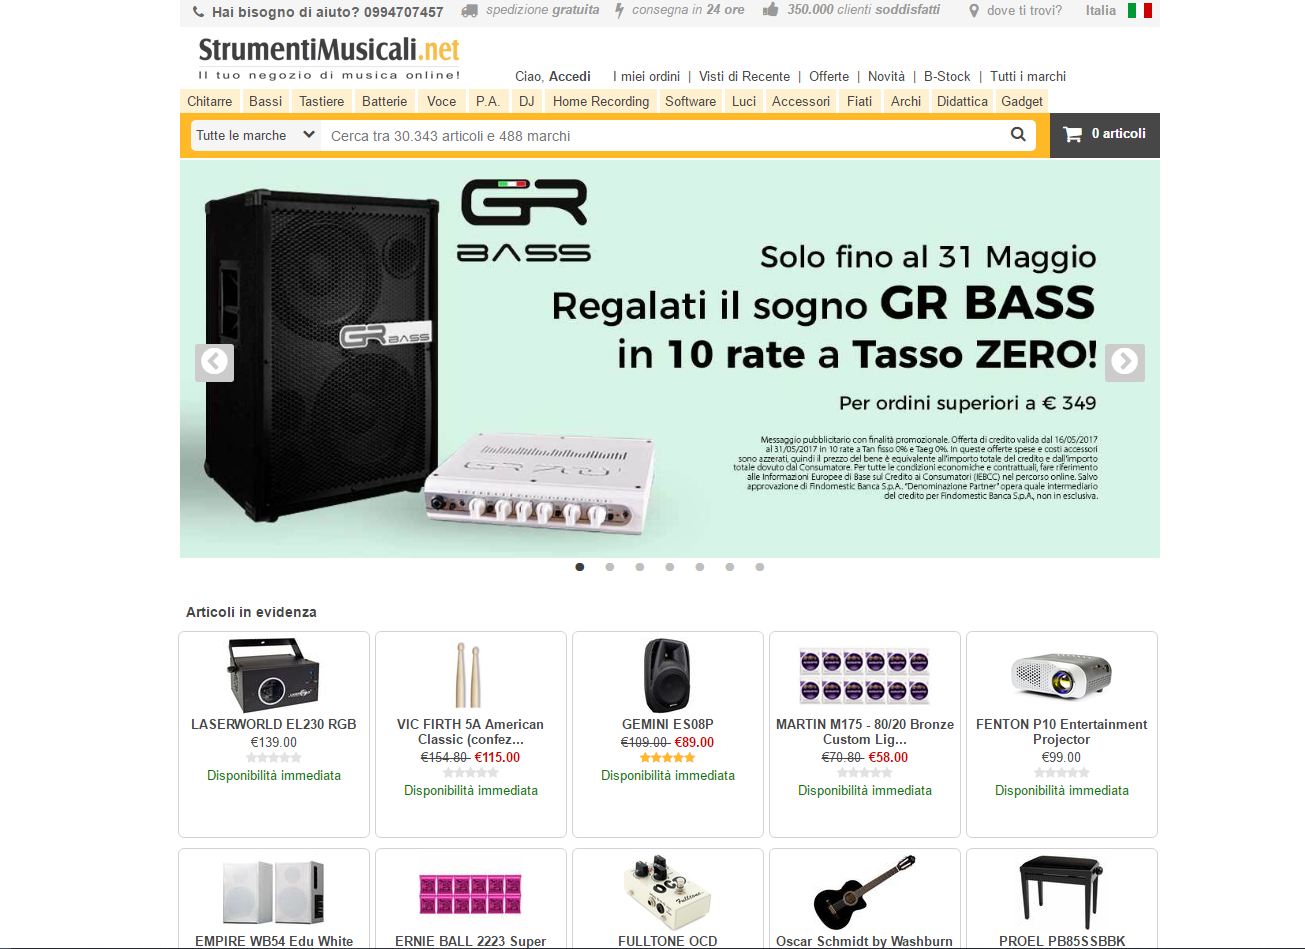
\includegraphics[width=150mm]{images/home.png}
		\caption{Homepage scroll 1}
	\end{figure}
	\begin{figure}
		\centering	
		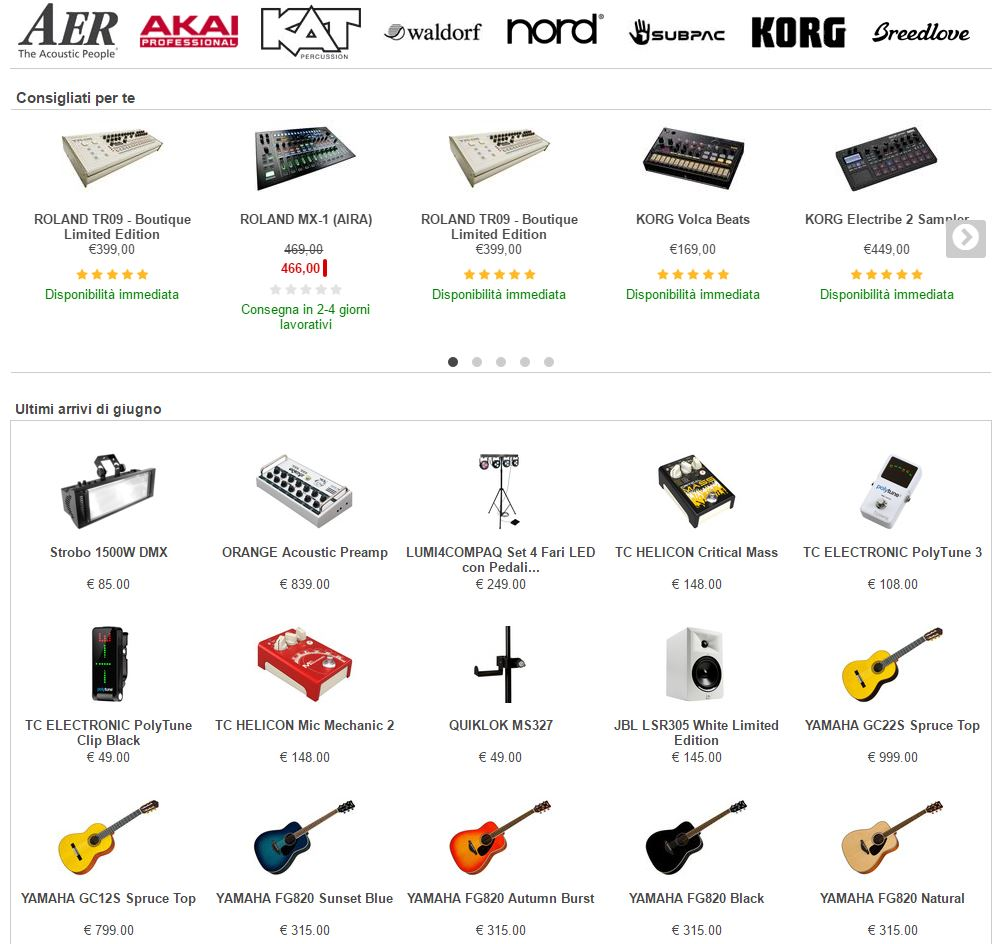
\includegraphics[width=150mm]{images/home2.png}%
		\caption{Homepage scroll 2}
	\end{figure}
	\begin{figure}
		\centering	
		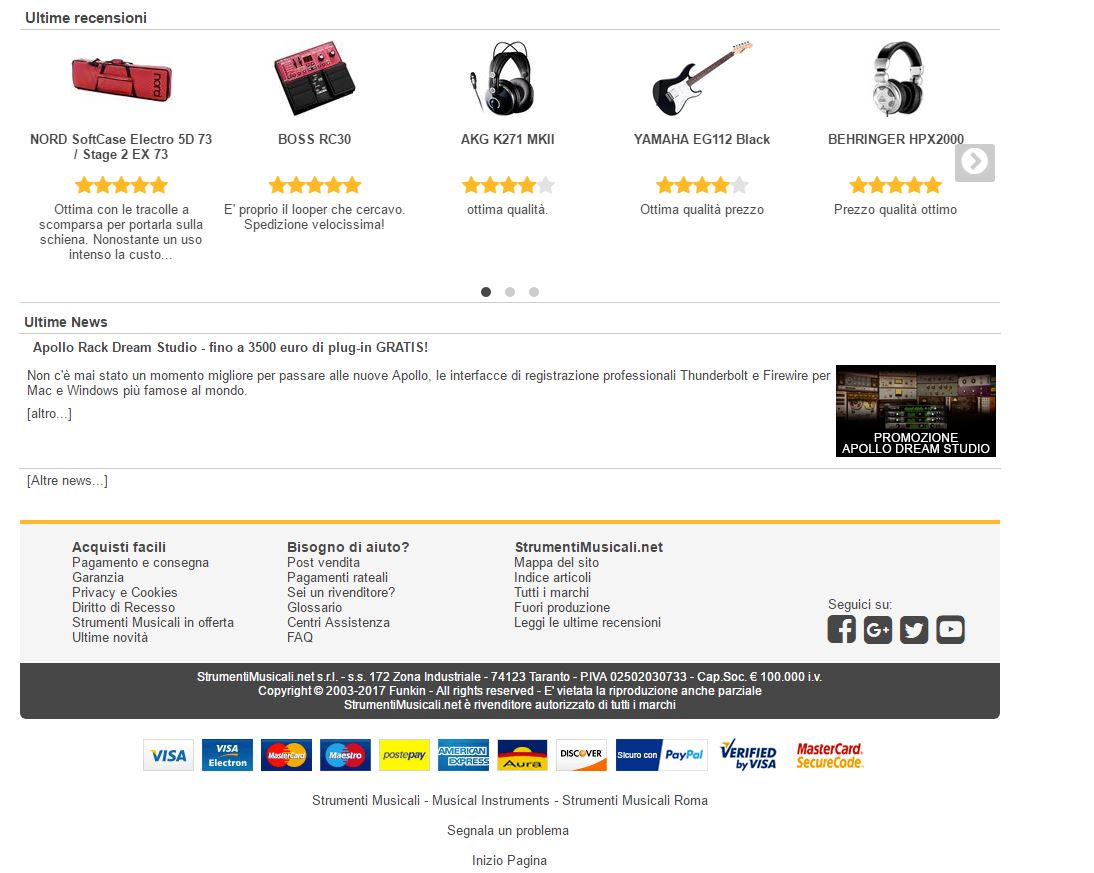
\includegraphics[width=150mm]{images/home3.png}%
		\caption{Homepage scroll 3}
	\end{figure}
	\newpage
	\subsection{Assi fondamentali}
	\vspace{0.5cm}
	Per prima cosa cerco di analizzare la pagina e provo a immedesimarmi nell'utente che visita per la prima volta il sito. Riesce a capire in che sito è finito? E trova quello che stava cercando?  Queste e altre domande fanno parte delle 6W che caratterizzano gli assi fondamentali di una pagina web.
	\paragraph{1) Where} "Dove mi trovo? In che sito sono arrivato? "
	\\ 
	A prima vista si nota subito che è un sito di strumenti e accessori musicali, lo slideshow in primo piano mostra diversi prodotti musicali, come casse audio e chitarre. Non è difficile capire che è un sito che vende strumenti musicali, nel logo notiamo la scritta "Il tuo negozio di musica online", inoltre possiamo vedere gli articoli in evidenza che presentano prezzo e disponiblità.
	\paragraph{2) What} "Cosa offre il sito? Cosa posso trovare? "
	\\
	L'indice del sito lo possiamo trovare in alto sotto il logo del sito. L'indice mostra le varie categorie di prodotti che offre, come chitarre, bassi, software e accessori.. \\ Nello slideshow vengono mostrati vari articoli, come novità o prodotti in notevole sconto, se clicchiamo nello slideshow verremo reindirizzati alla pagina del prodotto. Sotto lo slideshow è presente la sezione degli articoli in evidenza.
	\paragraph{3) Who} "Chi rappresenta il sito? "
	\\
	In alto a sinistra possiamo notare il logo del sito dell'azienda, punto importante per l'utente che permette di identificare il nome del sito. Se clicco sopra il logo ho solamente un refresh della home. Le informazioni dell'azienda le possiamo trovare nel footer dopo diversi scroll. 
	\paragraph{4) Why} "Perchè dovrei fermarmi su questo sito? Quali benefici mi porta?"
	\\
	Il perchè dovrei acquistare su questo sito non è visibile, però facendo un confronto dei prezzi che possiamo trovare in altri siti web o negozi fisici, si nota che ha dei prezzi pari o inferiori su quasi tutti i prodotti, risparmiando così diversi soldi. Inoltre è un sito specializzato con una vasta gamma di prodotti che difficilmente si può trovare in altri negozi.
	\paragraph{5) When} "Quali sono le novità del sito? "
	\\
	Le novità del sito le possiamo trovare sopra il menù nella sezione "Novità", cliccandoci sopra verremo reindirizzati alla pagina interna di tutti i nuovi articoli inseriti nel sito. Possiamo filtrare gli articoli in base alla categoria che ci interessa e ordinarli per prezzo crescente/decrescente o in ordine alfabetico. \\
	I nuovi arrivi li possiamo trovare anche nello slideshow, magari con una promozione e più sotto dopo un paio di scroll è presente la sezione degli ultimi arrivi del mese.
	\paragraph{6) How} "Come navigo nel sito? Come arrivo a quello che mi interessa? "
	\\
	Per navigare nel sito possiamo usare il menu per accedere alle varie categorie, è menu di tipo hover e se ci passo sopra con il mouse si apre una tendina con le varie sottocategorie. \\
	E' presente anche una grande barra di ricerca, ben riconoscibile dall'utente per via della lente (la metafora visiva viene quindi rispettata), che ci permette di trovare un qualsiasi prodotto.
\end{document}
